\documentclass[../../main.tex]{subfiles}
\begin{document}

\begin{flushright}
  \footnotesize\textit{【自動文字起こし・要確認】}
\end{flushright}

% Source: handwritten.pdf 第1問．
{\bf [解]}
\begin{align}
  \overrightarrow{OP}&=(1-s)
  \begin{pmatrix}3\\0\\0
  \end{pmatrix}
  +s
  \begin{pmatrix}3\\0\\4
  \end{pmatrix}
  =
  \begin{pmatrix}3\\0\\0
  \end{pmatrix}+s
  \begin{pmatrix}0\\0\\4
  \end{pmatrix},\\
  \overrightarrow{OQ}&=(1-t)
  \begin{pmatrix}0\\2\\0
  \end{pmatrix}
  +t
  \begin{pmatrix}0\\2\\4
  \end{pmatrix}
  =
  \begin{pmatrix}0\\2\\0
  \end{pmatrix}+t
  \begin{pmatrix}0\\0\\4
  \end{pmatrix}.
\end{align}
だから，$AC$上の点$R$を
\begin{align}
  \overrightarrow{OR}=\alpha
  \begin{pmatrix}3\\0\\0
  \end{pmatrix}
  +(1-\alpha)
  \begin{pmatrix}0\\2\\0
  \end{pmatrix}
  =
  \begin{pmatrix}0\\2\\0
  \end{pmatrix}+\alpha
  \begin{pmatrix}3\\-2\\0
  \end{pmatrix}
  \quad(0\leqq\alpha\leqq1)
\end{align}
で定めて，$DR\perp OP$かつ$DR\perp OQ$なる$\alpha$の存在条件をもとめれば良い．
\begin{figure}[H]
  \centering
  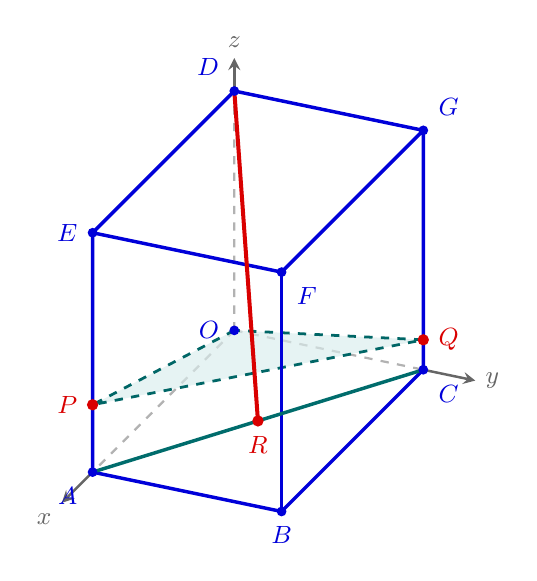
\begin{tikzpicture}[x={(-0.6cm,-0.6cm)}, y={(1.2cm,-0.25cm)}, z={(0cm,0.76cm)},
    >=stealth, every node/.style={font=\small}]
    \coordinate (O) at (0,0,0);
    \coordinate (A) at (3,0,0);
    \coordinate (B) at (3,2,0);
    \coordinate (C) at (0,2,0);
    \coordinate (D) at (0,0,4);
    \coordinate (E) at (3,0,4);
    \coordinate (F) at (3,2,4);
    \coordinate (G) at (0,2,4);
    % 9s/16 = 1-4t = 1/2 とした，条件を満たす配置例．
    \coordinate (P) at (3,0,1.125);
    \coordinate (Q) at (0,2,0.5);
    \coordinate (R) at (1.5,1,0);

    % 奥に隠れる稜線と，平面 OPQ を先に描く．
    \draw[dashed, gray!60, line width=0.8pt] (O)--(A) (O)--(C) (O)--(D) (B)--(F);
    \fill[teal!15, opacity=0.65] (O)--(P)--(Q)--cycle;
    \draw[dashed, teal!80!black, line width=1pt] (O)--(P)--(Q)--cycle;

    % 直方体の手前の稜線．
    \draw[blue!85!black, line width=1.25pt]
    (A)--(B)--(C)--(G)--(F)--(E)--(A) (E)--(D)--(G);
    \draw[blue!85!black, line width=1.25pt] (F)--(B);

    % 条件に現れる線分 AC と，D からの垂線の方向．
    \draw[teal!85!black, line width=1.25pt] (A)--(C);
    \draw[red!85!black, line width=1.45pt] (D)--(R);

    \draw[->, gray!80!black, line width=0.9pt] (A)--(3.65,0,0) node[below left] {$x$};
    \draw[->, gray!80!black, line width=0.9pt] (C)--(0,2.55,0) node[right] {$y$};
    \draw[->, gray!80!black, line width=0.9pt] (D)--(0,0,4.55) node[above] {$z$};

    \foreach \point/\position in {
      O/left,A/below left,B/below,C/below right,D/above left,
    E/left,F/below right,G/above right} {
      \node[circle, fill=blue!85!black, inner sep=1.25pt] at (\point) {}; \node[blue!85!black, \position=2pt] at (\point) {$\point$};
    }
    \foreach \point/\position in {P/left,Q/right,R/below} {
      \node[circle, fill=red!85!black, inner sep=1.45pt] at (\point) {}; \node[red!85!black, \position=2pt] at (\point) {$\point$};
    }
  \end{tikzpicture}
  \caption{直方体と点$P,Q,R$，平面$OPQ$の位置（模式図）}
\end{figure}
\begin{align}
  \overrightarrow{DR}=
  \begin{pmatrix}0\\2\\-4
  \end{pmatrix}
  +\alpha
  \begin{pmatrix}3\\-2\\0
  \end{pmatrix}
\end{align}
から
\begin{align}
  \overrightarrow{DR}\cdot\overrightarrow{OP}
  &=
  \begin{pmatrix}3\\0\\4s
  \end{pmatrix}\cdot
  \begin{pmatrix}3\alpha\\2-2\alpha\\-4
  \end{pmatrix}=0,\\
  \overrightarrow{DR}\cdot\overrightarrow{OQ}
  &=
  \begin{pmatrix}0\\2\\4t
  \end{pmatrix}\cdot
  \begin{pmatrix}3\alpha\\2-2\alpha\\-4
  \end{pmatrix}=0.
\end{align}
よって
\begin{align}9\alpha-16s=0,\qquad1-\alpha=4t.
\end{align}
だから$\alpha=\dfrac{16}{9}s=1-4t$であり，$0<s<1$，$0<t<1$から，この時常に$0<\alpha<1$となるので，
\begin{align}\dfrac{16}{9}s+4t=1.
\end{align}

\end{document}
